\documentclass{beamer}
\usepackage{amsmath}
\usepackage{amssymb}
\usepackage{graphicx}
\usepackage{gvv}
\usepackage{url}
\usetheme{Madrid}

\title{\textbf{7.4.12}}
\author{\textbf{Aditya Mishra — EE25BTECH11005}}
\date{October 12, 2025}

\begin{document}

\begin{frame}
\titlepage
\end{frame}

\begin{frame}{Question}
The centres of a set of circles, each of radius \(3\), lie on the circle \(x^2 + y^2 = 25\).
Find the locus of any point \(\vec{x}\) in the set.
\end{frame}

\begin{frame}{Solution}
For a circle,
\begin{align}
\vec{u} = -\vec{c}, \quad f = \|\vec{u}\|^2 - r^2
\end{align}
Hence, the general equation is
\begin{align}
\|\vec{x}\|^2 + 2\vec{u}^T\vec{x} + f = 0
\end{align}
For this family, since the centre lies on a circle, $\|\vec{u}\|=5$, $r=3$, $f=25-9=16$. Thus, any point on such a circle satisfies
\begin{align}
\|\vec{x}\|^2 + 2\vec{u}^T\vec{x} + 16 = 0
\end{align}
\end{frame}

\begin{frame}{Solution}
\begin{align}
2\vec{u}^T\vec{x} = -\|\vec{x}\|^2 - 16
\end{align}
Since \(\|\vec{u}\| = 5\), by Cauchy-Schwarz Inequality:
\begin{align}
-5\|\vec{x}\| \le \vec{u}^T\vec{x} \le 5\|\vec{x}\|
\end{align}
\end{frame}

\begin{frame}{Solution}
The minimum value of \(2\vec{u}^T\vec{x}\) is \(-10\|\vec{x}\|\).  
Hence, existence requires
\begin{align}
-10\|\vec{x}\| \le -\|\vec{x}\|^2 - 16
\end{align}
\end{frame}

\begin{frame}{Solution}
\begin{align}
\|\vec{x}\|^2 - 10\|\vec{x}\| + 16 \le 0
\end{align}
\begin{align}
2 \le \|\vec{x}\| \le 8
\quad \Rightarrow \quad
4 \le \vec{x}^T\vec{x} \le 64
\end{align}
\[
\boxed{4 \le x^2 + y^2 \le 64}
\]
\end{frame}

\begin{frame}{Figure}
    \centering
    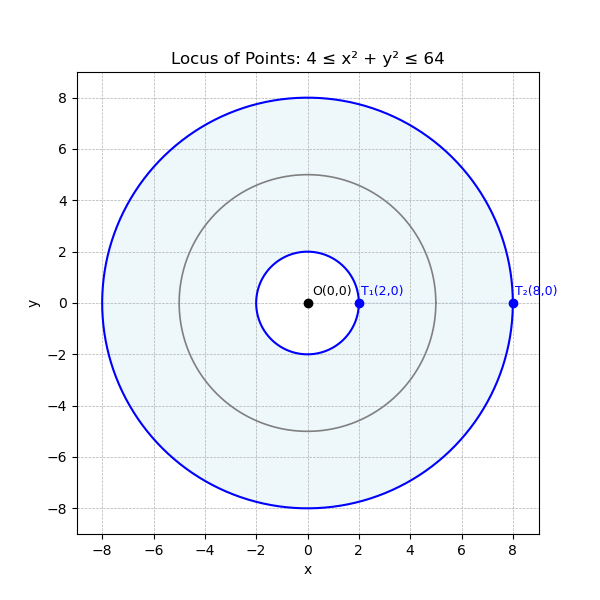
\includegraphics[width=0.6\columnwidth]{Figs/Figure_1.png}
    \\[4pt]
    {\small Plot of the locus of points for circles of radius 3 with centers on $x^2 + y^2 = 25$.}
\end{frame}

\begin{frame}{Codes}
\centering
For Codes, refer to:  
\url{https://github.com/Aditya-Mishra11005/ee1030-2025/tree/main/ee25btech11005/matgeo/7.4.12/Codes}
\end{frame}

\end{document}

